\chapter{CO observations of star-forming regions}
\label{ch:chapter3}

\section{Introduction to CO contamination and outflows}

\section{HARP}

\section{CO reduction}

\section{CO observations}

\subsection{PPV Clouds}
\subsection{Outflows}


\section{CO contamination of SCUBA-2 850\,$\micron$}

\subsection{Literature}

%Previous studies of contamination of CO [INTRO]
CO is known to be found in conjunction with dust and molecular hydrogen gas in GMCs, 
either in the form of ambient ground or excited states. Observing bright CO is used to 
trace either high column densities of molecular gas (assuming the emission is optically thin) 
or heating through exposure to radiative feedback. Careful analysis of line emission profile 
can be used to identify outflows which are the signatures of embedded protostars \citep{Graves:2010mb}. 
Outflows primarily provide dynamical feedback into a molecular cloud, though the most 
powerful outflows may also contribute a small, localised radiative component.

We use our HARP 345.796\,GHz observations of the $^{12}$CO 3\hbox{--}2 line emission 
to assess the impact of CO emission on the 850\,$\micron$ band, which is a known contaminant 
of the 850\,$\micron$ band  \citep{Gordon:1995uq} observed by SCUBA-2.  

\cite{Davis:2000vn} and \cite{Tothill:2002ys} have all observed CO contamination of 
SCUBA data of up to 10\% whilst \cite{Hatchell:2009fk} have found contamination up 
to 20\%. \cite{Johnstone:2003ys} and \cite{Drabek:2012uq} record a minority of cases 
where CO emission dominates the dust emission (up to 79\%) in SCUBA-2 observations, 
with these regions hosting substantial molecular outflows in addition to ambient molecular 
gas within the clouds.

Given that CO contamination affects the 850\,$\micron$ band but not the 450\,$\micron$ band, 
an assessment of $^{12}$CO 3\hbox{--}2 line emission is vital for an accurate assessment of 
dust temperature with unaccounted CO emission producing artificially lower ratios and cooler 
temperatures (Equation \ref{eqn:temp}, see Section 5). We use \cite{Drabek:2012uq}'s method 
by which CO line integrated intensities can be converted into 850\,$\micron$ flux densities and 
directly subtracted from SCUBA-2 data. 

\subsection{Methodology}
%MWC 297
Reliable temperatures depend on accurate input fluxes. Systematic contamination of 450\,$\micron$ and 850\,$\micron$ flux 
by molecular lines, in particular CO, is a known problem within SCUBA-2 data \citep{Drabek:2012uq}. We investigate the contribution of CO and 
free-free emission to these bands and attempt to mitigate their effects where necessary.

\section{Contamination in the Serpens MWC 297}
%MWC 297
\cite{Hatchell:2013ij} and \cite{Drabek:2012uq} highlighted 345 GHz contamination of 850\,$\micron$ due to the CO~3\hbox{--}2 
line in other Gould Belt star-forming regions. Limited $^{12}$CO and $^{13}$CO~1\hbox{--}0 data exist for the Serpens 
MWC 297 region \citep{Canto:1984dq}. A very rough estimate of the CO contamination towards the star MWC 297 can be made 
based on the published spectra. The $^{12}$CO lines are broad ($\sim 12~\hbox{ km s}^{-1}$) but do not show line wings characteristic of 
outflows.  Making the simplest assumption that the $^{12}$CO is optically thick and fills the beam in both the $J=1\hbox{--}0$ 
and $J=3\hbox{--}2$ lines, the integrated intensity of the latter will be similar to the former, $\sim 36\,\hbox{K km s}^{-1}$, 
corresponding to a CO contamination of 1.14 mJy/pixel/K km$^{-1}$ (13\,per cent of peak flux) at the position of the star MWC 297 
using the conversion in \citet{Drabek:2012uq} updated for the beam parameters in \citet{Dempsey:2013uq}. \cite{Drabek:2012uq} 
noted than regions where CO emission accounts for less that 20\,per cent of total peak emission are not consistent with outflows or 
major contamination. \cite{Manoj:2007ly} find no evidence of CO~2\hbox{--}1 and $^{13}\textrm{CO~2\hbox{--}1}$ emission within 
80\,AU of MWC 297 and conclude this depletion is caused by photoionisation due to an ultra-compact \HII\ (UCH\textrm{II}) region 
as has been detected by \cite{Drew:1997qf} and \cite{Malbet:2007zr}. 

\cite{Fuente:2002dq} - high res 13CO + 18CO. Evidence of a cavity. 
\cite{Ridge:2003cr} - Low res 18CO. 



\section{Contamination in the the W40 complex}

\subsubsection{Observations}

%W40
Archival HARP $^{12}\textrm{CO}$ 3\hbox{--}2 data \citep{van-der-Wiel:2014vn} confirms 
the presence of red- and blue-shifted gas in the Dust Arc (Figure \ref{fig:maps}) but coverage 
is limited to a 2\arcmin\ $\times$ 2\arcmin\ region centred on the peak of the submilimetre 
emission, and therefore we commissioned an extended survey of the W40 complex in 
$^{12}\textrm{CO}$ 3\hbox{--}2 that included the whole of the Dust Arc and W40-N, as 
presented in Figures \ref{fig:maps} and \ref{fig:CO}. Subsequent to our observations, 
\cite{Shimoikura:2015kx} mapped the W40 complex the Atacama Submillimeter Telescope 
Experiment (ASTE) observations in $^{12}\textrm{CO}$ 3\hbox{--}2 and HCO$^{+}$ 
4\hbox{--}3 with a similar coverage, but at the lower effective resolution of 
22\arcsec\ compared to the JCMT (14.6\arcsec).

%W40
Aquila was observed with HARP (Heterodyne Array Receiver Programme, 
\citeauthor{Buckle:2009fk} \citeyear{Buckle:2009fk}) on the 4th of July 2015 as part of the 
M15AI31 "active star-formation in the W40 complex" proposal. The main beam efficiency, 
$\eta_{\mathrm{MB}}$, taken from the JCMT efficiency archive is 0.61 at 345\,GHz. Two 
sets of four basket-weaving scan maps were observed over an approximately 7\arcmin 
$\times$18\arcmin\ area (position angle = 65$^{\degr}$) at 345.796\,GHz to observe the 
$^{12}$CO 3\hbox{--}2 line. A sensitivity of 0.3\,K was achieved on 1\,km s$^{-1}$ velocity 
channels in weather Grade 4 ($\tau_{225}$ = 0.16). Maps were referenced against an 
off-source position at RA(J2000) = 18:33:29.0, Dec.(J2000) = -02:03:45.4, which had been 
selected as being free of any significant CO emission in the \cite{Dame:2001qf} CO 
Galactic Plane Survey. 

%W40
%The observed cube has two distinct velocity components at 5 and 10\,km\,s$^{-1}$ that 
%are consistent with \cite{Zeilik:1978qf} and \cite{Shimoikura:2015kx}. A third component 
%at 7\,km\,s$^{-1}$ is detected in  observations of HCO$^{+}$ 4\hbox{--}3 line. 
%\cite{Shimoikura:2015kx} suggests that $^{12}$CO 3\hbox{--}2 is heavily affected by 
%self-absorption by this third cloud component, making full analysis of velocity structure 
%of the W40 complex challenging.   

%W40
The data were first reduced using the {\sc smurf} \texttt{makecube} technique 
\citep{Jenness:2015fk}. An integrated intensity map, corrected for main beam efficiency, 
was produced by collapsing along the entire velocity range and subsequently run through 
the SCUBA-2 data reduction pipeline with the effect of filtering out scales larger than 
5\arcmin\ as well as regridding to 3\arcsec\ pixels. Figure \ref{fig:CO} presents the reduced 
$^{12}$CO 3\hbox{--}2 integrated intensity map for the W40 complex. 

\begin{figure*}
\begin{centering}
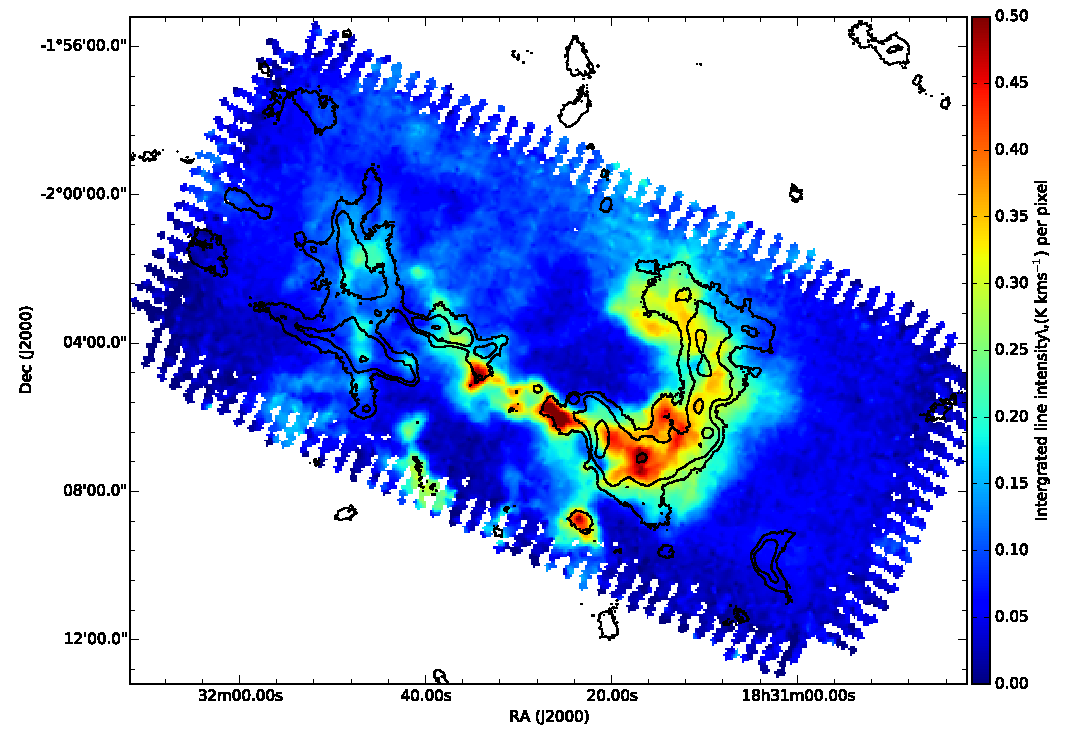
\includegraphics[scale=1]{c3/figs/20150805_W40_CO.pdf}
\caption{$^{12}$CO 3\hbox{--}2 integrated intensity map over the entire range (colour scale over -90 to +100\,km s$^{-1}$) of the central region of the W40 complex. Contours show SCUBA-2 850\,$\micron$ emission at the 5$\sigma$, 15$\sigma$ and 50$\sigma$ levels.} 
\label{fig:CO}
\end{centering}
\end{figure*} 


\subsubsection{Contamination results}

Integrated intensity maps of $^{12}\textrm{CO}$ 3\hbox{--}2 emission are subtracted from 
the original SCUBA-2 850\,$\micron$ maps using a joint data reduction process before a 
4\arcmin\ filter is applied following the method outlined in Appendix B. The fraction of 
SCUBA-2 emission that can be accounted for by $^{12}\textrm{CO}$ 3\hbox{--}2 line 
emission is presented in Figure \ref{fig:COconamination}. Contamination in W40-N is 
minimal with levels up to 5\%. The Dust Arc has significantly more contamination at the 
level of 10\%, reaching up to 20\% at its highest. 

Figure \ref{fig:COfilter} shows the distribution of flux ratios (Equation \ref{eqn:temp} and the method 
given in Appendix A) with and without CO contamination contributing to 850\,$\micron$, showing how 
even a small degree of CO contamination can have a significant effect on measuring the temperature 
of the cloud, increasing the modal flux ratio from 6.8 to 7.8 when CO is subtracted. Furthermore, the 
FWHM of the distribution increases from 1.9 to 2.8. Subtracting CO from our maps increases the 
mean and standard deviation of temperature in regions where $^{12}\textrm{CO}$ 3\hbox{--}2 is 
detected, in comparison with temperatures derived from uncorrected maps. The distribution of flux 
ratios across the map, with and without the CO contamination, are compared and found to have a 
KS-statistic of 0.253, corresponding to 1.3\% probability that the two samples are drawn from the 
same parent sample. CO contamination in the W40 complex is having a significant impact on 
distribution of flux ratios. 

\begin{figure}
\begin{centering}
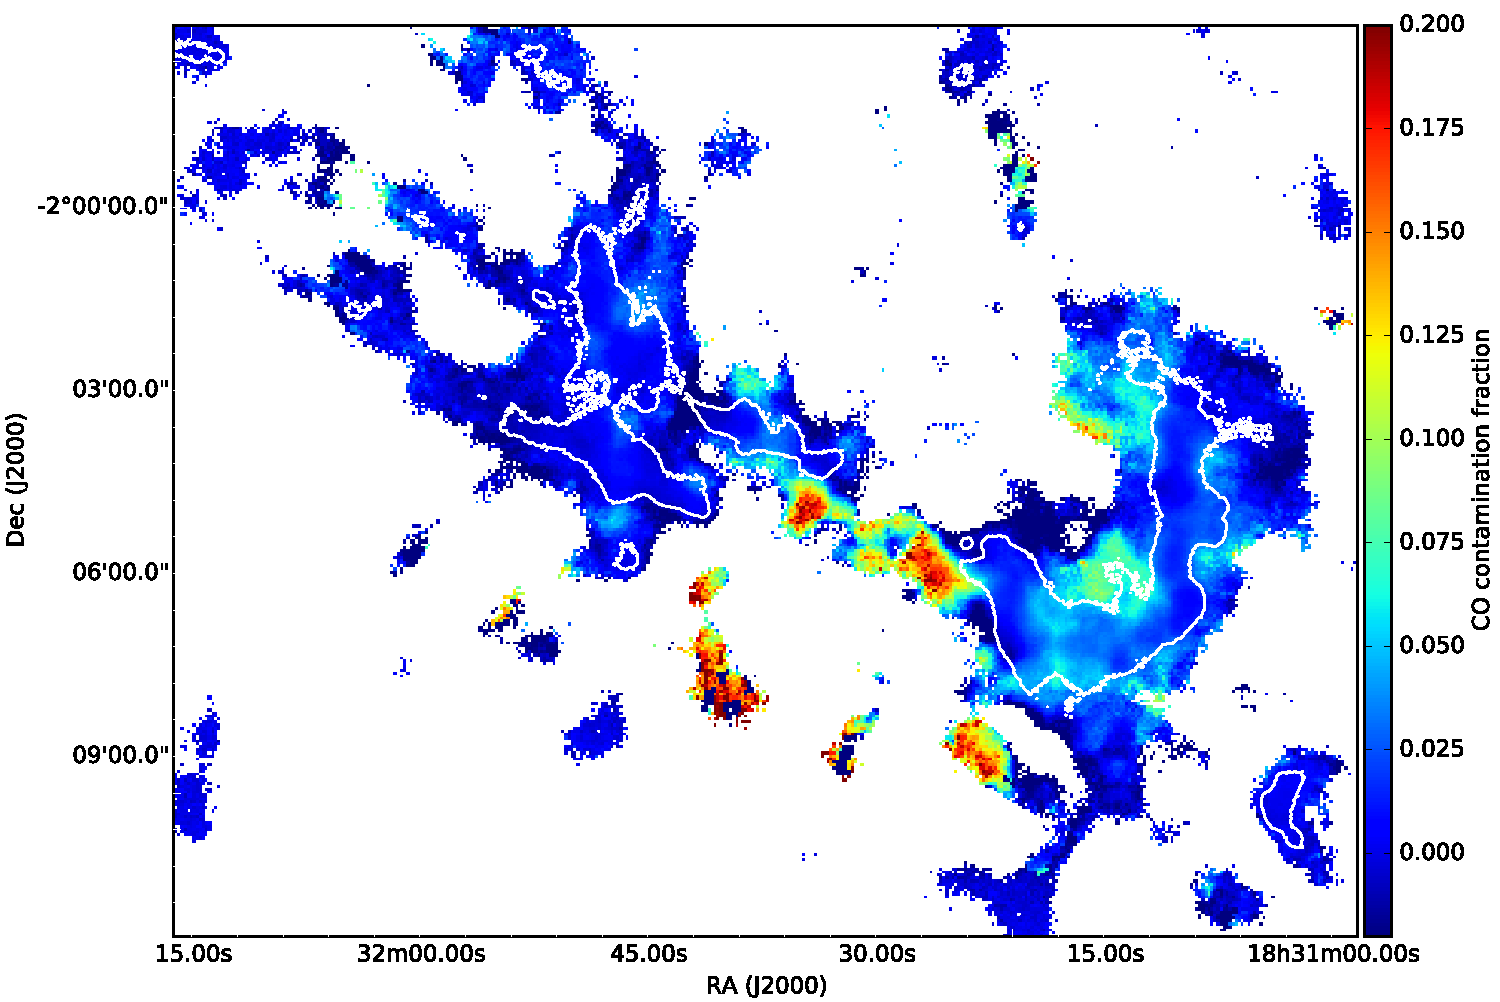
\includegraphics[scale=0.35]{c3/figs/20150804_COcontamination.pdf}
\caption{The fraction of SCUBA-2 850\,$\micron$ that can be attributed to $^{12}\textrm{CO}$ 3\hbox{--}2 345\,GHz line emission. The SCUBA-2 data are masked at 3$\sigma$ and the 5$\sigma$ level is shown in white.} 
\label{fig:COconamination}
\end{centering}
\end{figure} 

\begin{figure}
\begin{centering}
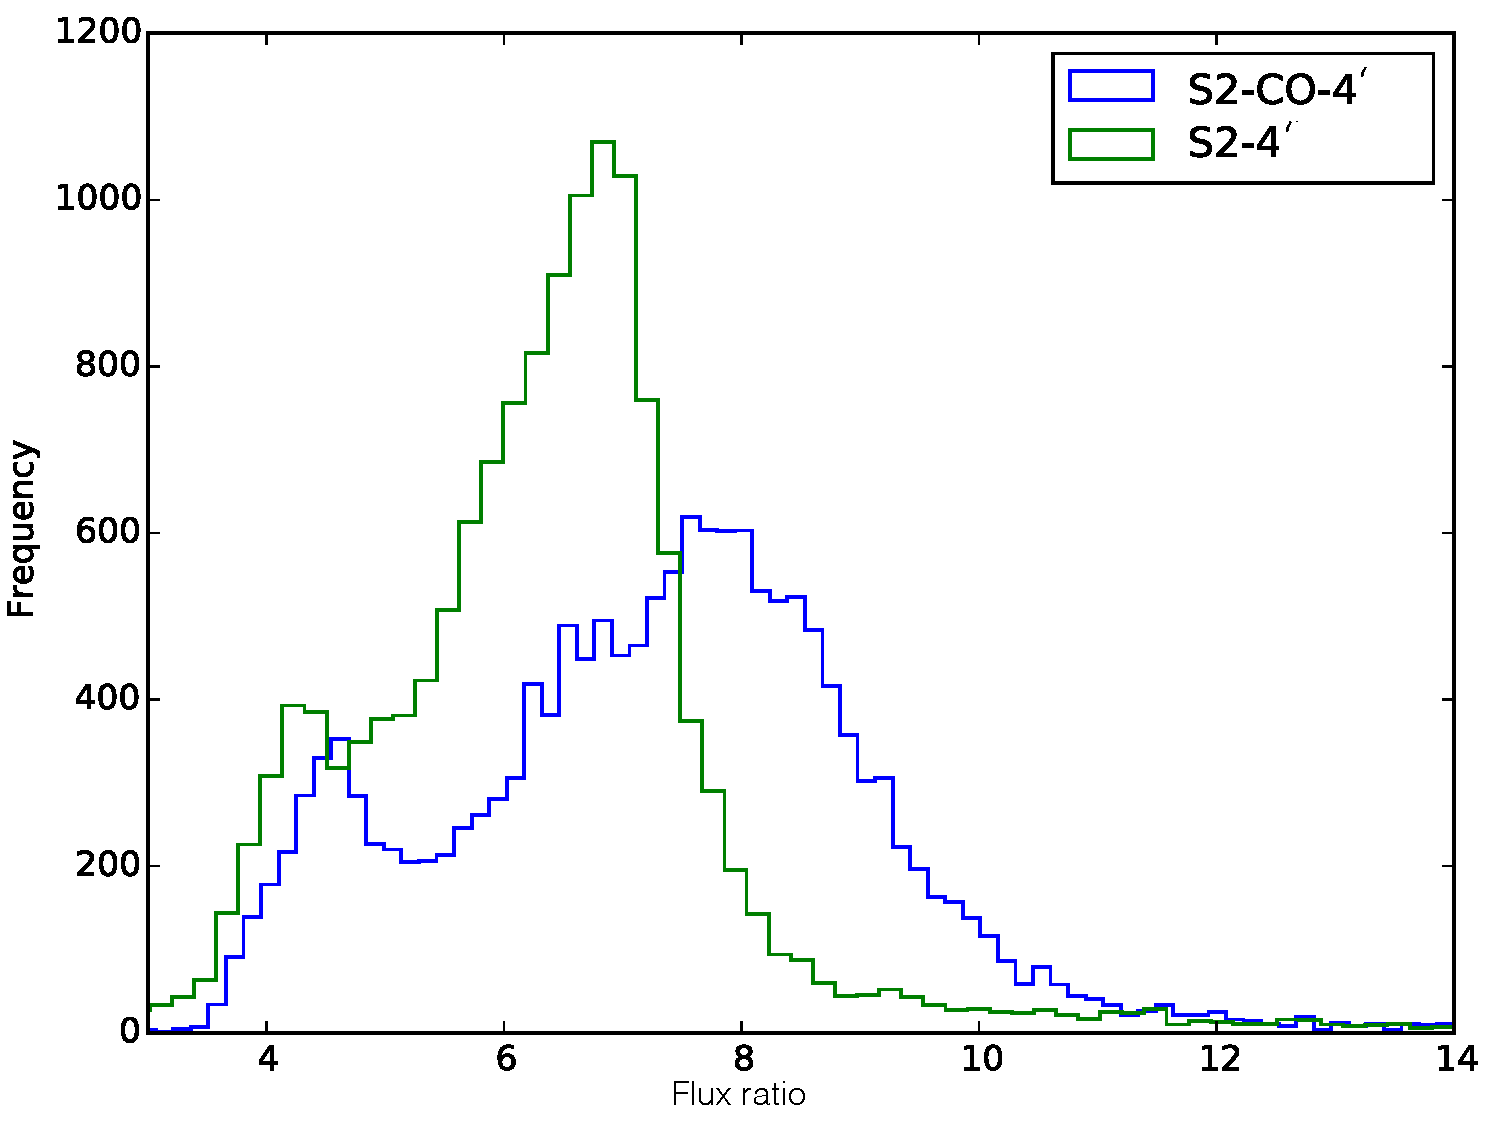
\includegraphics[scale=0.35]{c3/figs/20150804_KStest-conoco.pdf}
\caption{The distribution of 450\,$\micron$/850\,$\micron$ flux ratio for the original (blue - S2-4\arcmin) and CO subtracted (green - S2-CO-4\arcmin) Aquila reductions with additional 4\arcmin\ spatial filtering. KS-statistics reveal a 1.3\% chance that the two data sets are drawn from the same distribution.} 
\label{fig:COfilter}
\end{centering}
\end{figure} 


\subsection{Cloud velocities}

\begin{figure}
\begin{centering}
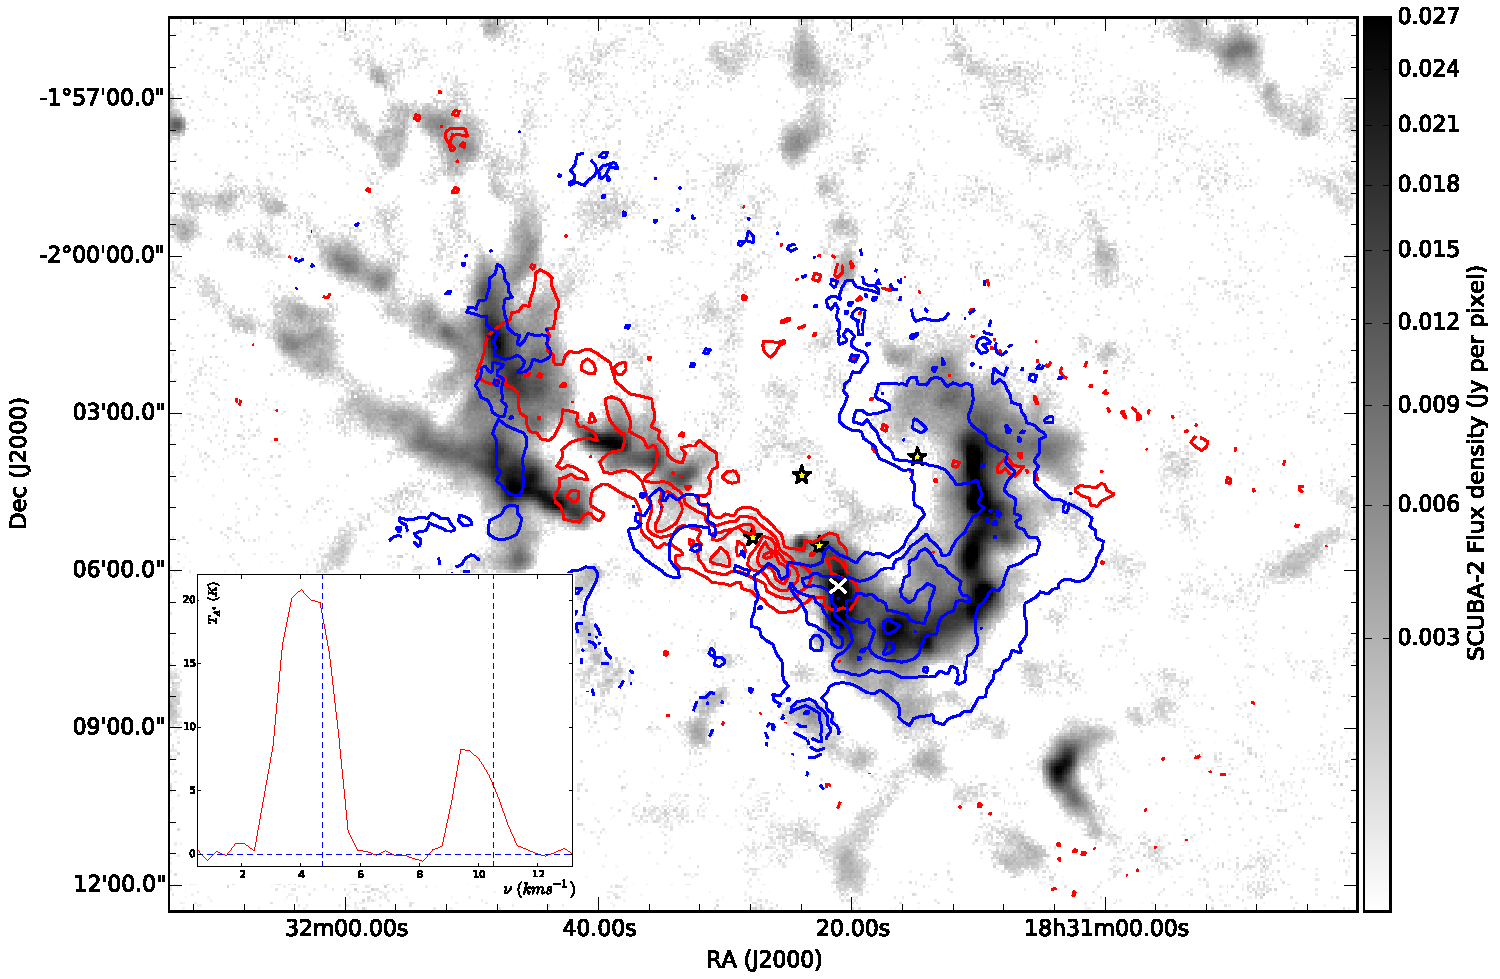
\includegraphics[scale=0.55]{c3/figs/20150904_twoclouds.pdf}
\caption{SCUBA-2 850\,$\micron$ map of the W40 complex with $^{13}\textrm{CO~2\hbox{--}1}$ integrated intensity contours of red (10km\,s$^{-1}$) and blueshifted (5km\,s$^{-1}$) emission that trace out the location of two separate clouds within the region. Blue contours are at 20, 40, 60, 80 K km\,s$^{-1}$ and red are the same levels with an additional contour at 5K km\,s$^{-1}$. The greyscale SCUBA-2 850\,$\micron$ shown here has not had CO emission subtracted. Yellow stars mark the location of the OB stars in the W40 complex. The insert shows the line emission spectra at the position of peak SCUBA-2 luminosity, marked with a white cross. Two CO clouds are visible at 5 and 10 km\,s$^{-1}$ with a significant vacancy at 7 km\,s$^{-1}$ where Shimoikura et al. 2015 finds $\textrm{HCO~4\hbox{--}3}$ emission, indicating that our $^{13}\textrm{CO~2\hbox{--}1}$ absence is due to optical depth and self-absorption.} 
\label{fig:2clouds}
\end{centering}
\end{figure} 


Two distinct components are visible in the velocity space of the $^{13}\textrm{CO~2\hbox{--}1}$ cube and are presented in Figure D1. A blueshifted component is observed at approximately 5km\,s$^{-1}$ (consistent with Zeilik & Lada 1978 and Shimoikura et al. 2015) with peak integrated flux of 88K km\,s$^{-1}$ that is coincident with the SCUBA-2 emission in the Dust Arc and, to a lesser extent, W40-N. A redshifted component is observed at approximately 10 km\,s$^{-1}$ with an integrated flux of 86 K km\,s$^{-1}$ and tightly traces a low luminosity filament of SCUBA-2 emission between W40-N and the Dust Arc, passing through the location of the OB association in the W40 complex.

Atacama Submillimeter Telescope Experiment (ASTE) observations by \cite{Shimoikura:2015kx} provides evidence of a third velocity of approximately 7 km\,s$^{-1}$ observed in $\textrm{HCO~4\hbox{--}3}$ at the submilimetre peak of the cloud (their Figure 2). $\textrm{HCO~4\hbox{--}3}$ remains optically thin at high column densities where $^{13}\textrm{CO~2\hbox{--}1}$ may become optically thick. \cite{Shimoikura:2015kx} argue that the sharp partition between 5 and 10km\,s$^{-1}$, as seen in the insert of Figure D1, may be due a dense cloud at 7 km\,s$^{-1}$ in which $^{13}\textrm{CO~2\hbox{--}1}$ is extincted but $\textrm{HCO~4\hbox{--}3}$ is observed.

Our observations of 5 and 10 km\,s$^{-1}$ $^{13}\textrm{CO~2\hbox{--}1}$ componentsare consistent with \cite{Shimoikura:2015kx}'s interpretation of a molecular shell, swept up and heated by the expanding \HII\ region, with divergent velocities either side of the shell. We find less evidence to support their claim that the ambient gas in the W40 complex has a velocity of 7 km\,s$^{-1}$ as we detect no $^{13}\textrm{CO~2\hbox{--}1}$ at that velocity in the relatively low density filaments that are significantly outside of the \HII\ shell. It is unlikely that this component extends to our off position (RA (J2000) = 18:33:29.0, Dec. (J2000) = -02:03:45.4) as it was throughly examined in \cite{Zeilik:1978qf}'s $^{12}\textrm{CO~1\hbox{--}0}$ observations and found to be clear.

HARP data are found to contain two clouds at 5 km\,s$^{-1}$ and 10km\,s$^{-1}$ that trace different morphological structures (Figure D1). The redshifted filament starts in W40-N and traces a line from this cloud to the tip of the Dust Arc. The emission from $^{13}\textrm{CO~2\hbox{--}1}$ is observed in SCUBA-2 850\,$\micron$ data and closely fits the HARP data, albeit at high SNRs, as shown in Figures D1 and 19. The red filament passes directly through the stellar cluster, enveloping the location of OS1a and the \HII\ region, as shown in Figure 19.

Since CO is photo-dissociated in \HII\ regions, the red filament is either shielding CO gas from the UV photons, or it is located in the foreground or background of the \HII\ region. SCUBA-2 does not detect a significant dust filament coincident with redshifted the CO and therefore we discount the former premise. Furthermore, figure 19 shows how clumps W40-SMM 12, 13, 20, 21, 23 and 39 are coincident both with the bright rimmed clouds (BRCs) observed in Herschel 70\,$\micron$ data and peaks of redshifted CO emission, confirming that the CO gas is within the nebulosity. This picture is consistent with the findings of \cite{Shimoikura:2015kx} who suggested the redshifted filament is a shell of heated CO gas swept up in the expanding shockwave around the \HII\ region.

\subsection{Outflow analysis}

\begin{figure*}
\begin{centering}
\begin{tabular}{l}
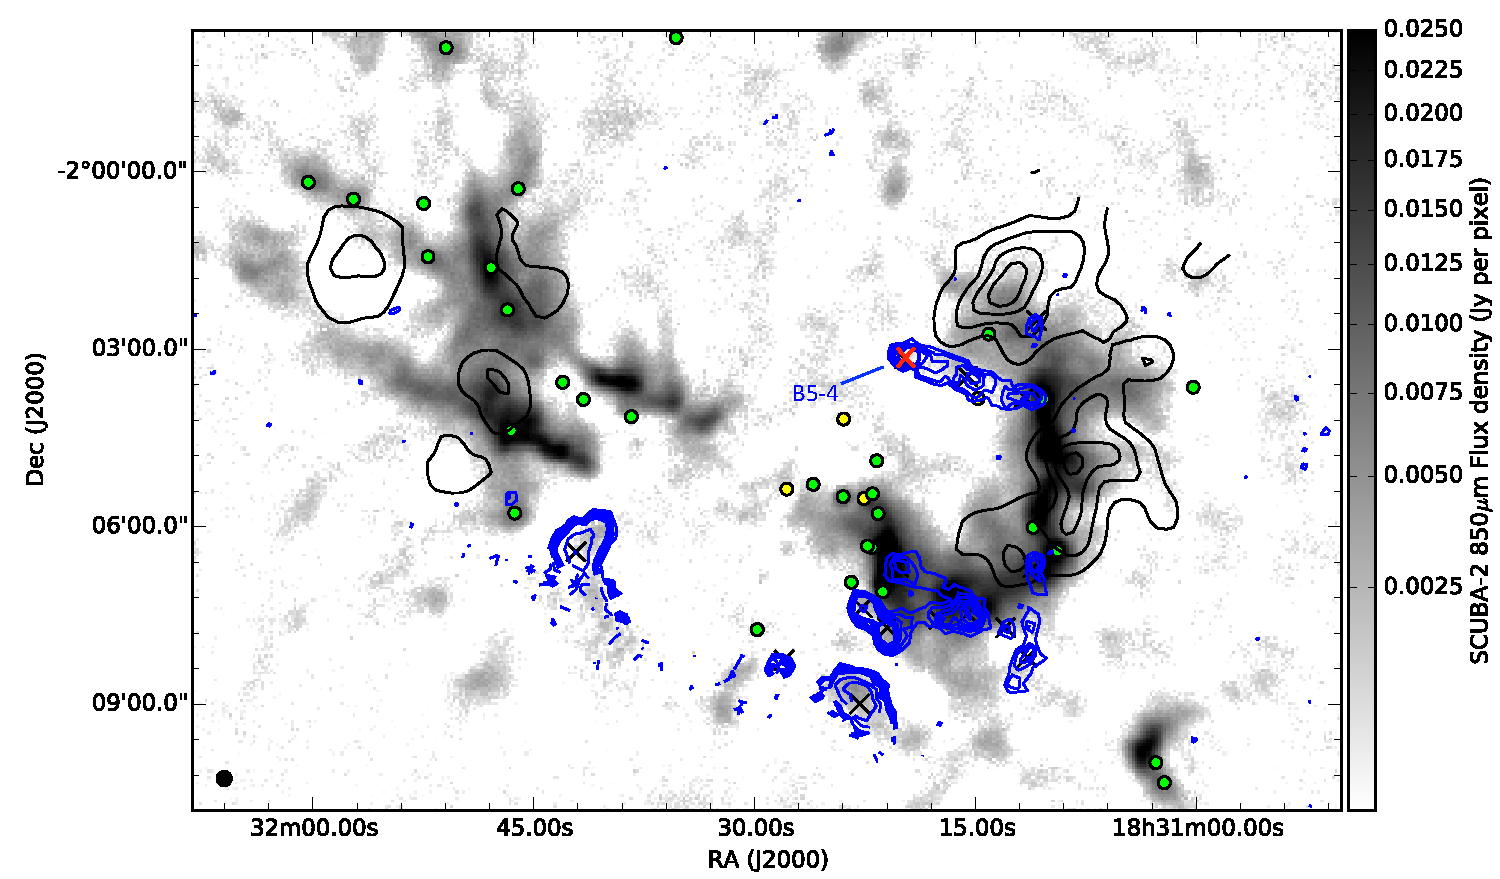
\includegraphics[scale=0.55]{c3/figs/20150903_5kmsoutflow_map.pdf} &
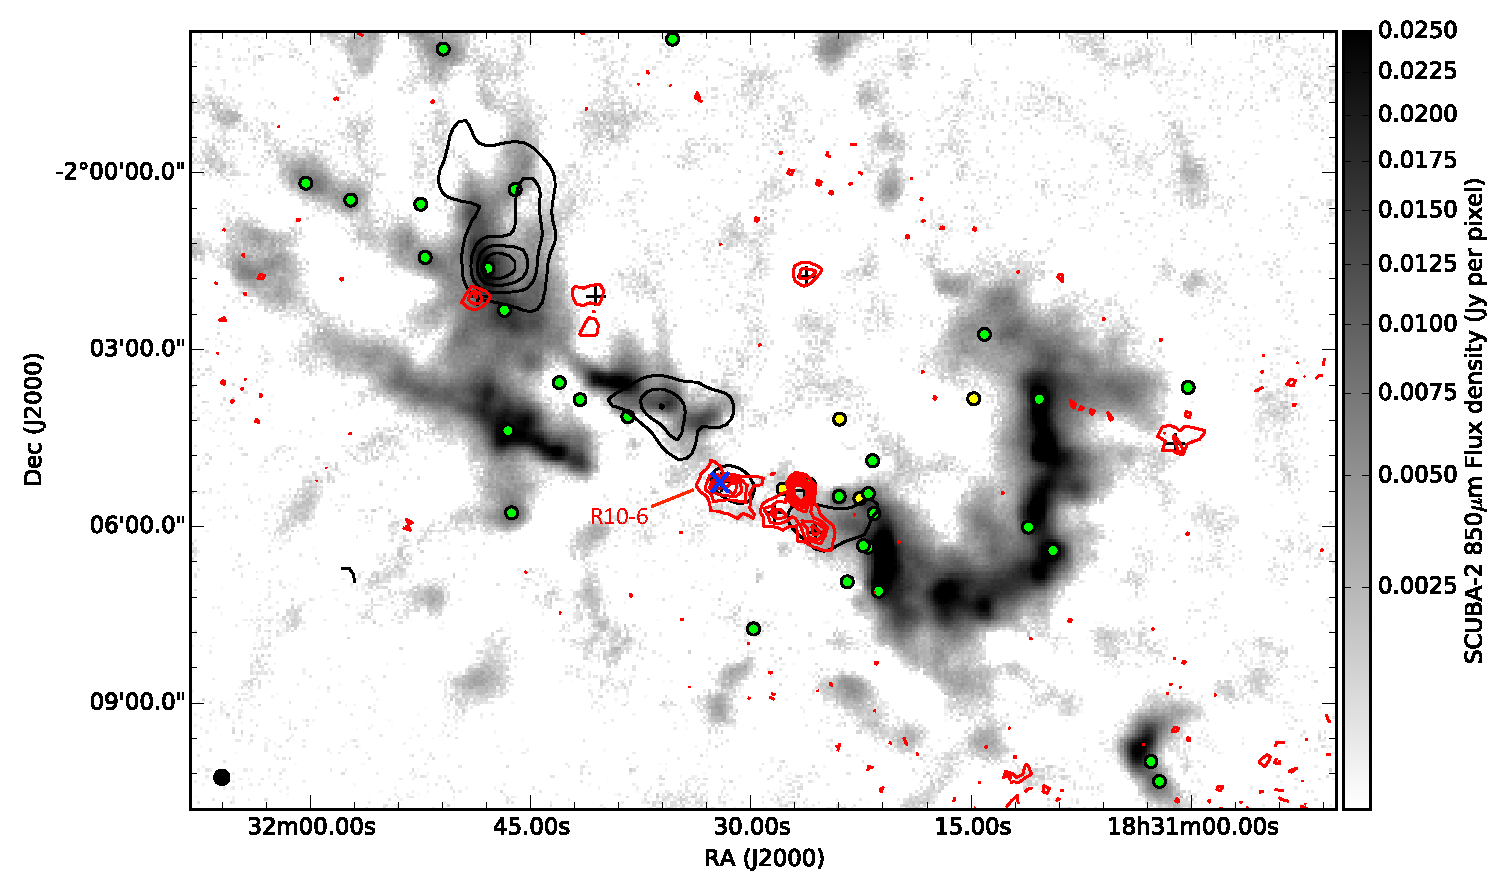
\includegraphics[scale=0.55]{c3/figs/20150903_10kmsoutflow_map.pdf} &
\end{tabular}
\caption{2CO 3�2 integrated line emission in the blue wing of the 5 km\,s$^{-1}$ (upper), and red wing of the 10\,km\,s$^{-1}$ cloud (lower). The blue 5\,km\,s$^{-1}$ wing is integrated over the velocity range 3.2$\leq$v$_{LSR}$$\leq$2.8km\,s$^{-1}$. The red 10\.km\,s$^{-1}$ wing is integrated over the velocity range 11.7$\leq$v$_{LSR}$$\leq$14.5\,km\,s$^{-1}$. Line wing sources are identified from local peaks in emission, identified as black crosses in the respective plots. Yellow stars and green circles indicate the location of the OB stars and protostars (from our composite YSOc catalogue). The grayscale backdrop map is SCUBA-2 850\,$\micron$ flux density. The black, smoothed contour represents emission from the alternative line wing (see text for velocity ranges).}
\label{fig:linewings}
\end{centering}
\end{figure*} 

\begin{figure*}
\begin{centering}
\begin{tabular}{l}
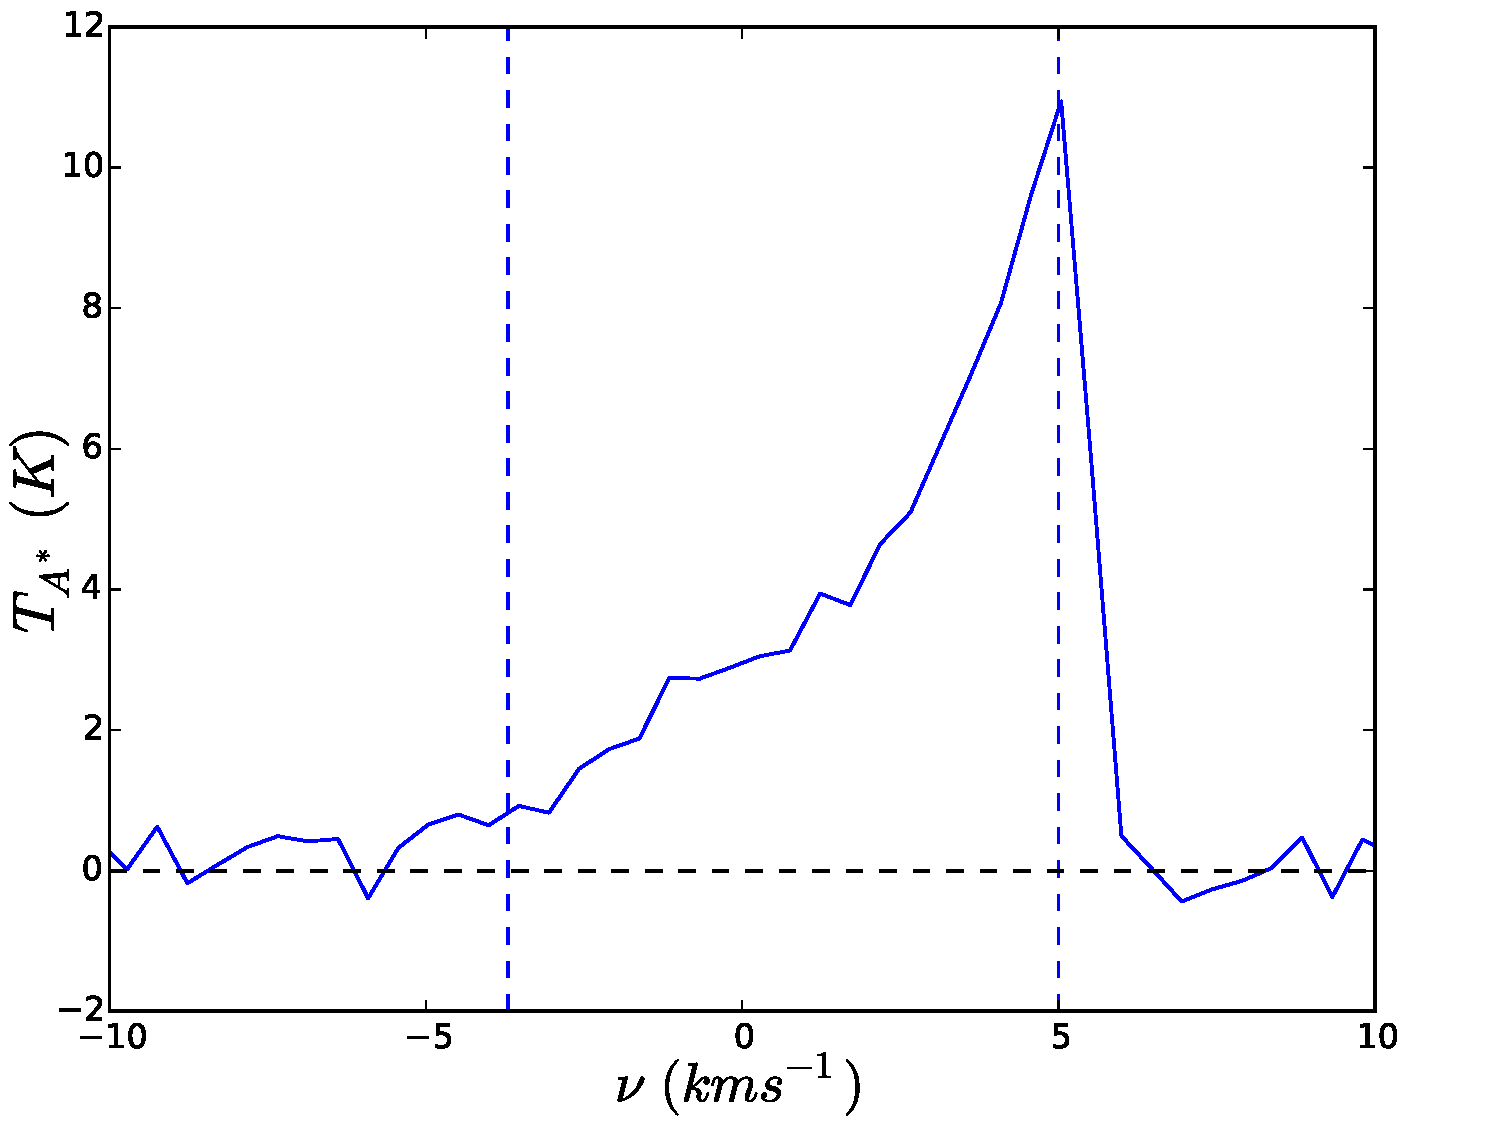
\includegraphics[scale=0.3]{c3/figs/B5-4outflow.pdf}
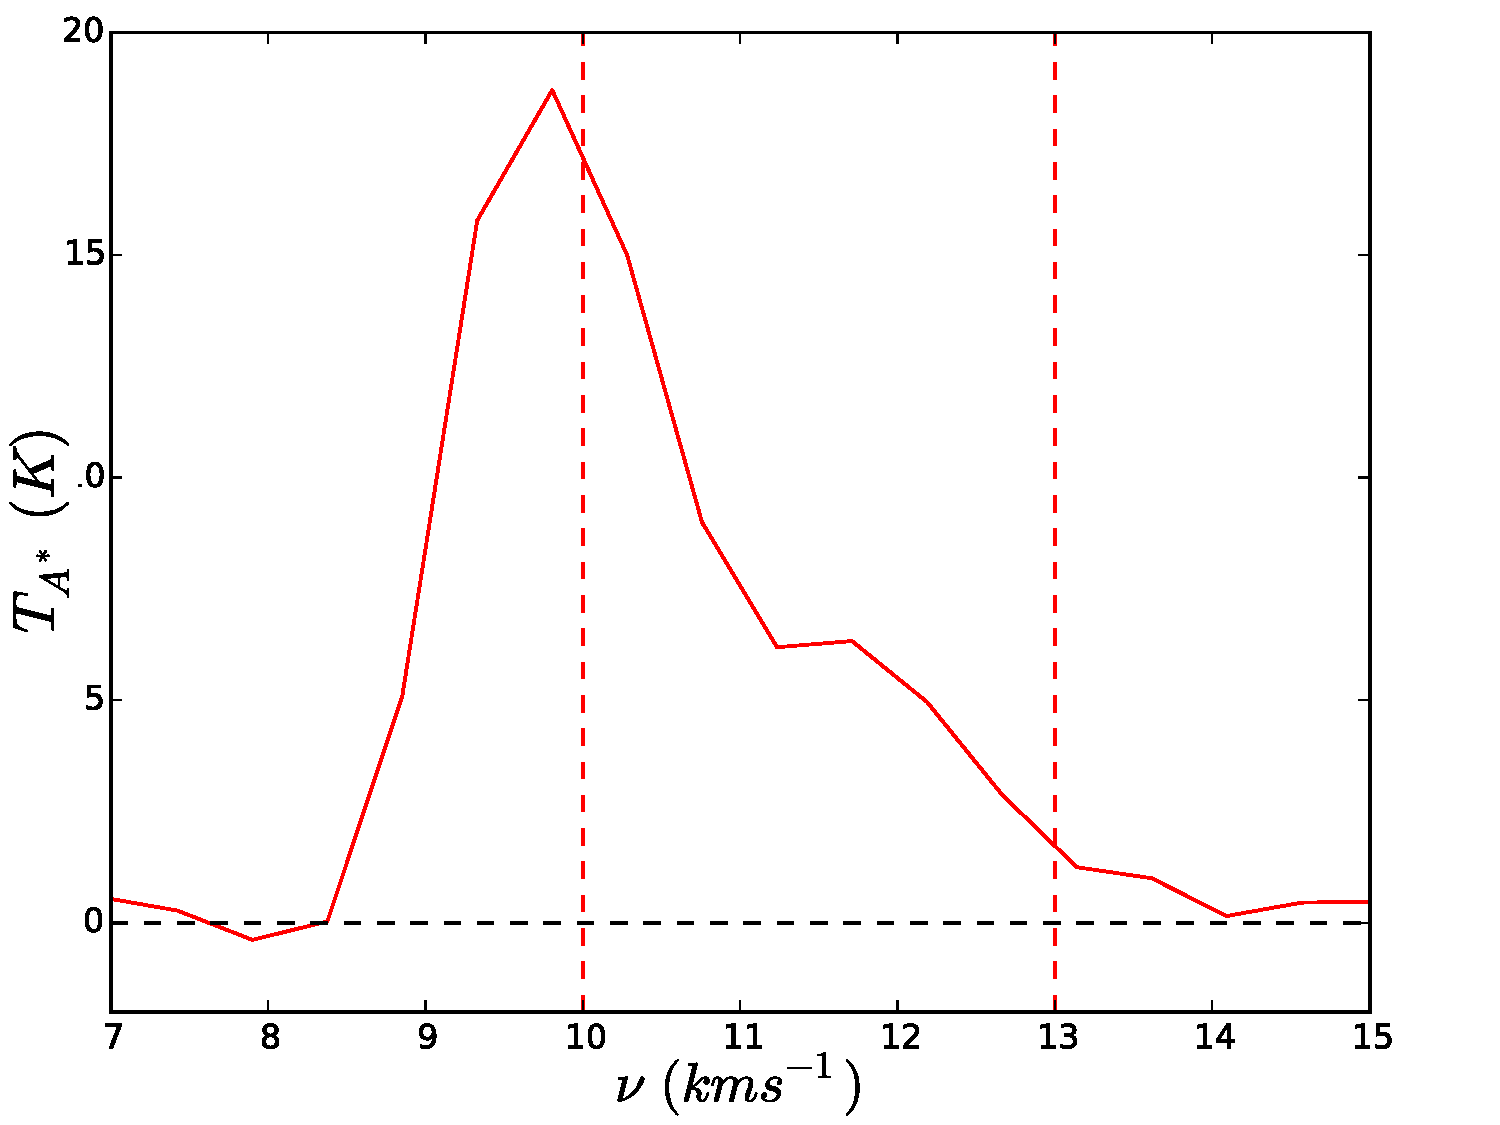
\includegraphics[scale=0.3]{c3/figs/R10-6outflow.pdf}
\end{tabular}
\caption{$^{13}\textrm{CO~2\hbox{--}1}$ line profiles of example outflows R10-6 (left) and B5-4 (right) with their locations in the 10 and 5 km\,s$^{-1}$ clouds respectively marked in Figure E1. Each profile shows prominent outflow line-wings that are either red or blue shifted. Dotted lines demonstrate the length of the line-wing, from local cloud velocity to its maximum extent.}
\label{fig:outflowslines}
\end{centering}
\end{figure*} 

A first wave of $^{12}\textrm{CO~1\hbox{--}0}$ observations of the W40 complex was made by \cite{Zeilik:1978qf} who found an ambient cloud with extended emission symptomatic of outflows with a local standard of rest velocity across the region of approximately 4.5km\,s$^{-1}$. Evidence of a weak molecular outflow was found by \cite{Zhu:2006ee}.

The complex nature of redand blue-shifted emission in the W40 complex makes direct analysis of individual outflows very difficult. We instead refer to the method of identifying local peaks in $^{13}\textrm{CO~2\hbox{--}1}$ integrated over the velocity ranges redand blue-ward of the 5 km\,s$^{-1}$ and 10 km\,s$^{-1}$ components, respectively, as used by \cite{Shimoikura:2015kx}. Peaks can be used to identify molecular outflows from protostars where the line profile shows a line-wing similar to those observed by \cite{Graves:2010mb} in Serpens Main. This method is also sensitive to the bulk motion of shocked gas around the shell of the \HII\ region, local variations in ambient gas velocity and foreground clouds at different velocity. Multiple outflow features in the �outer' velocity ranges (-3.2$\leq$v$_{LSR}$$\leq$2.8 km\,s$^{-1}$ and 11.7$\leq$v$_{LSR}$$\leq$14.5 km\,s$^{-1}$) are detected (Figure E1). The `inner' regions (5.7$\leq$v$_{LSR}$$\leq$8.4 km\,s$^{-1}$ and 8.5$\leq$v$_{LSR}$ $\leq$9.2 km\,s$^{-1}$) are where paired outflows would be expected, however \cite{Shimoikura:2015kx} outlines how $^{13}\textrm{CO~2\hbox{--}1}$ emission becomes optically thick due to a dense cloud at 7km\,s$^{-1}$, and subsequently heavily extincts any outflows in this region of the spectrum.

We detect 15 blue objects in the 5 km\,s$^{-1}$ component and nine red objects in the 10 km\,s$^{-1}$ component. These detections are almost twice the number detected by \cite{Shimoikura:2015kx}, primarily as a result of the higher resolution of the JCMT. Of this total, five are confirmed as outflows using the criterion of \cite{Hatchell:2007ly}, whereby the line wing is required to have an intensity greater than 3$\sigma$ at $\pm$3km\,s$^{-1}$ from the bulk cloud. The two most significant outflows of each cloud are presented in Figure E2. R10-6 and B5-4 have linewing widths of 3.5 km\,s$^{-1}$ 8.7 km\,s$^{-1}$, respectively. A further seven candidate outflows have a notable asymmetry in their line profiles but have too much noise to be confirmed. Eight objects are displaced components with no line asymmetries or wing-like features. Three are noise artefacts or have very low SNRs.

Of the 12 outflow-like detections, 11 have nearby protostars identified in our composite YSO catalogue (Figure E1). Due to the complexity of the region and lack of observations from the �inner' wings of the cloud it would be premature to infer that the completeness of our Class 0/I protostellar population is near 100\%. We conclude that the 10 km\,s$^{-1}$ CO filament is likely shocked shell material around the \HII\ region and we cannot rule this shell out as a source of many of the weaker candidate outflows near OS1a and IRS 5.
There is evidence that significantly powerful protostellar outflows can contribute additional localised heating of dust through shocks \citep{Buckle:2015vn}. Outflows have been detected in the W40 complex by \cite{Zeilik:1978qf} and more recently \cite{van-der-Wiel:2014vn} found red and blue shifted line wings in the eastern Dust Arc. Our HARP data extend this coverage to the whole of the Dust Arc and W40-N (Figure 3).

We detect 12 potential molecular outflows which are presented in Figure E1. The highest velocity line-wing offset is 8.7km\,s$^{-1}$ and is recorded in outflow B5-4 which is associated with a protostar in W40-SMM2. Line-wings found in Serpens Main by \cite{Graves:2010mb} are detected out to -30 km\,s$^{-1}$ and +37 km\,s$^{-1}$ from an ambient cloud of similar velocities to the W40 complex. We conclude that the outflows in the W40 complex are relatively weak and that the radiative heating from outflows is negligible, relative to the levels of the radiative feedback from the protostar itself.

We conclude that many of the line-wing detections in Figure E1 are likely caused by shocks related to this wave as opposed to protostellar outflows.

Some of the most prominent outflows we detect are found in the western Dust Arc. For example, Figure E1 shows the outflow B5-4 subtending 3\arcsec\ (0.43 pc) in length from the the protostar W40-MM5 \citep{Maury:2011ys} in W40-SMM3. As discussed in Section 6.1[UPDATE], the size of these linewings are not particularly exceptional. Given a clump mass of 12.5$\pm$2.6\,M$_{\odot}$ , we would anticipate low-to-intermediate mass star-formation is occurring. W40-SMM2 is the only significant clump in the western Dust Arc that does not have a protostar recorded in our composite YSO catalogue. In addition, no significant CO line-wing emission is detected, suggesting that this clump is indeed starless.

The $^{13}\textrm{CO~2\hbox{--}1}$ emission (Figure E1) shows many line-wing sources to the north and south of W40-SMM1 from both the 5 and 10 km\,s$^{-1}$ clouds. It is not possible to assign individual outflows to protostars, or to rule out that the line-wings could be caused by shocked gas swept up in a shell where the \HII\ region interacts with the filament. The absence of CO line-wing sources in the vicinity of the YSOs near OS2b does suggest that either; these are particularly low-mass protostars with weak outflows, the majority of the $^{13}\textrm{CO~2\hbox{--}1}$ has been photo-ionised by the \HII\ region, or that the protostars detected here are false detections.

\section{Conclusions}


\begin{enumerate}
\item We find evidence for significant levels of $^{12}$CO 3\hbox{--}2 line emission in 
HARP data that contaminates the 850\,$\micron$ band range between 3 and 10\% in 
the majority of the filaments. In a minority of areas contamination reaches up to 20\%. 
Removing the $^{12}$CO 3\hbox{--}2 contamination significantly increases the 
calculated dust temperatures, beyond the calculated uncertainties. 
\end{enumerate}